\section{Results and discussion}
\label{sec:results}

\subsection{The no-LLM baseline, and the pipeline against it}\label{sec:baseline}

Every accuracy number in this work is read against one reference, stated before any of our own: the
sandbox the pipeline is built on, mapping its own signature hits to ATT\&CK technique identifiers
deterministically, with no language model anywhere. Table~\ref{tab:results-1} reports it together
with the like-for-like comparison against the pipeline.

\begin{table}[!htbp]
\caption{The no-LLM baseline, and the pipeline against the engine it is built on. Both blocks are scored per sample against family-level MITRE ground truth by the same code; intervals resample families, not samples.}\label{tab:results-1}
\centering\small
\begin{tabular}{@{}lrrrr@{}}
\toprule
& mean & 95\% cluster CI & ICC & effective n \\
\midrule
\multicolumn{5}{@{}l}{\emph{baseline alone, n=\fact{baseline-n} samples over \fact{baseline-families} families}} \\
precision & \fact{baseline-precision} & \fact{baseline-precision-cluster-ci} & \fact{baseline-precision-icc} & \fact{baseline-precision-effective-n} \\
recall & \fact{baseline-recall} & \fact{baseline-recall-cluster-ci} & \fact{baseline-recall-icc} & \fact{baseline-recall-effective-n} \\
F1 & \fact{baseline-f1} & \fact{baseline-f1-cluster-ci} & \fact{baseline-f1-icc} & \fact{baseline-f1-effective-n} \\
\midrule
\multicolumn{5}{@{}l}{\emph{paired, n=\fact{h2h-n} samples over \fact{h2h-families} families, F1}} \\
CAPE alone, no language model & \fact{h2h-cape-f1} & \fact{h2h-cape-ci} & & \\
pipeline, static evidence only & \fact{h2h-static-f1} & \fact{h2h-static-ci} & & \\
pipeline, with the sandbox report & \fact{h2h-dynamic-f1} & \fact{h2h-dynamic-ci} & & \\
\bottomrule
\end{tabular}
\end{table}

The baseline block covers \fact{baseline-n} samples over \fact{baseline-families} families, mean
\fact{baseline-mean-cluster} samples per family, with the bootstrap seed recorded alongside the
interval. CAPE asserted at least one technique on every sample, so this is a predictor rather than
an artefact of an empty one. Ground truth is resolved per family, so two binaries of one family are
scored against a byte-identical label vector and are not two observations; resampling samples rather
than families gave an F1 interval \fact{baseline-f1-widening} times narrower on data whose
intra-cluster correlation is \fact{baseline-f1-icc}, which is why the row count is
\fact{baseline-n} and the count that supports an inference is \fact{baseline-f1-effective-n}.

Three analyst agents, a negotiation loop, a revision pass, an LLM judge and a weighted corroboration
cascade land \fact{h2h-delta} F1 from the signature engine they are built on top of, 95\% cluster CI
\fact{h2h-ci}, exact cluster sign-flip p = \fact{h2h-p-exact}, better on \fact{h2h-better} of
\fact{h2h-n}. Two of the means agreeing to four decimal places is a coincidence, and was checked
rather than reported: the samples differ individually in both directions, so the system is not
reproducing the sandbox's answers but reaching different answers of the same quality. The interval
is what should be read rather than the point. At \fact{h2h-families} families this design could
detect a difference of \fact{h2h-mde} F1 at 80\% power and did not detect one, which bounds the
pipeline's contribution rather than demonstrating that it is zero.

The cohort is \fact{baseline-n} rather than \fact{audit-tasks} because the sandbox reported every task of the submitted batch complete and \fact{audit-instant} of them had not run at all. Re-submitting recovered \fact{audit-recovered}; the mechanism and the timing evidence are reported as the fifth boundary case in Section~\ref{sec:failures}.

\begin{figure}
\centering
\pandocbounded{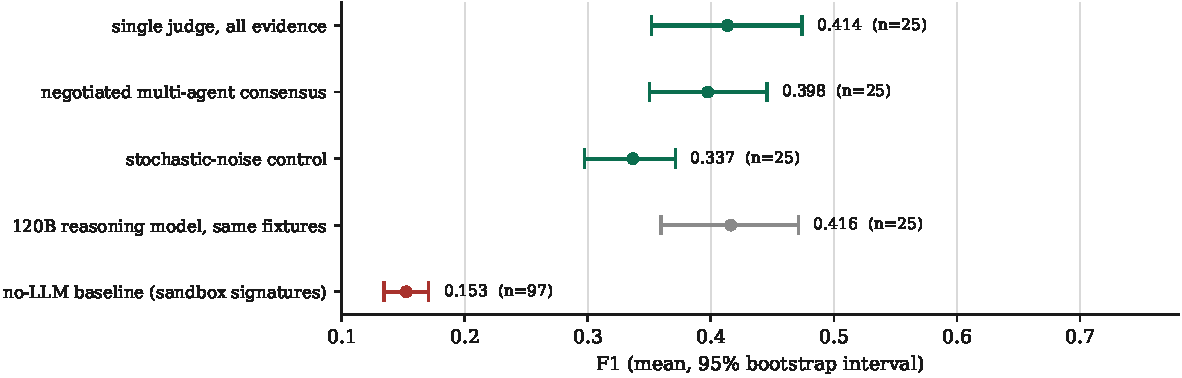
\includegraphics[keepaspectratio,alt={Figure 1: every measured arm on one F1 axis. Panel a) is the synthesised fixtures, panel b) the real-sample population where pipeline and baseline are comparable.}]{figures/fig3-arms-against-baseline.pdf}}
\caption{Every measured arm on one F1 axis. a) the synthesised fixtures, b) the real-sample population. Points are means over per-sample F1, bars are 95\% intervals resampling the cluster the observations are independent at.}
\end{figure}

The two panels of Figure~1 deliberately do not share an axis. An earlier version put all five arms
on one scale, where a no-LLM baseline near \fact{baseline-f1} beneath treatment arms near
\fact{consensus-single-f1} read as a large pipeline win. It is not one: panel a)'s arms run on
\fact{fixture-clusters} synthesised fixtures whose evidence is generated from their own technique
lists and are scored against per-sample truth, while the baseline runs on real binaries scored
against family-level truth. No baseline is definable for panel a) at all, since a deterministic
regular expression over the dictionary that generated its evidence scores
\fact{fixture-extractor-f1} there by construction. Panel b) is the comparison that can be made, and
its three intervals overlap.

\subsection{Multi-agent consensus at equal budget}\label{sec:consensus}

Three arms at an equal total token budget, including a stochastic-noise control in which one analyst
receives irrelevant evidence, run first on the fixtures and then again on real binaries one per
family so that every cluster holds a single observation. Table~\ref{tab:results-3} reports both.

\begin{table}[!htbp]
\caption{The equal-budget consensus arms, on synthesised fixtures and on real binaries. The real-sample block is scored against the same family-level ground truth as Table~\ref{tab:results-1}; the fixture block is not comparable to it.}\label{tab:results-3}
\centering\small
\begin{tabular}{@{}lrrrr@{}}
\toprule
arm & mean F1 & rows & output tokens & $\times$ single \\
\midrule
\multicolumn{5}{@{}l}{\emph{\fact{fixture-clusters} synthesised fixtures}} \\
single judge, all evidence at once & \fact{consensus-single-f1} & \fact{consensus-single-n} & & \\
negotiated multi-agent consensus & \fact{consensus-negotiated-f1} & \fact{consensus-negotiated-n} & & \fact{consensus-token-ratio} \\
noise control & \fact{consensus-noise-f1} & \fact{consensus-noise-n} & & \\
\midrule
\multicolumn{5}{@{}l}{\emph{\fact{cape-consensus-families} real samples, one per family}} \\
single judge & \fact{cape-consensus-single-f1} & \fact{cape-consensus-single-calls} & \fact{cape-consensus-single-tokens} & \fact{cape-consensus-single-ratio} \\
negotiated consensus & \fact{cape-consensus-negotiated-f1} & \fact{cape-consensus-negotiated-calls} & \fact{cape-consensus-negotiated-tokens} & \fact{cape-consensus-negotiated-ratio} \\
noise control & \fact{cape-consensus-noise-f1} & \fact{cape-consensus-noise-calls} & \fact{cape-consensus-noise-tokens} & \fact{cape-consensus-noise-ratio} \\
\bottomrule
\end{tabular}
\end{table}

On the fixtures the negotiated arm returns a paired delta against the single judge of
\fact{consensus-negotiated-delta}, 95\% cluster CI \fact{consensus-negotiated-ci}, an interval
containing zero, at \fact{consensus-token-ratio}$\times$ the tokens. This design could have detected
\fact{mde-consensus-negotiated} F1 at 80\% power and the observed difference is two orders of
magnitude smaller, so the null is a bound on what the design could see rather than a demonstration
of equivalence. The noise control moves by \fact{consensus-noise-delta},
\fact{consensus-noise-ci}, with every one of the \fact{fixture-clusters} samples in the same
direction, but that effect is also below the design's own minimum detectable effect of
\fact{mde-consensus-noise} and the exact cluster permutation test returns p =
\fact{consensus-noise-p-exact}, the smallest p available, because at \fact{fixture-clusters}
clusters the two-sided sign-flip test floors at \fact{fixture-signflip-floor}. An earlier draft read
that separation as proof of sensitivity; it does not carry that weight, and the honest statement is
that all \fact{fixture-clusters} samples moved the same way.

The real-sample replication is where the design can see. At \fact{cape-negotiated-k} clusters the
sign-flip floor is \fact{cape-negotiated-p-floor} rather than \fact{fixture-signflip-floor}. Both
multi-agent arms beat the single judge and neither beats the other: negotiated minus single is
\fact{cape-negotiated-delta}, 95\% cluster CI \fact{cape-negotiated-ci}, q =
\fact{cape-negotiated-q-exact}, better on \fact{cape-negotiated-better} of
\fact{cape-negotiated-pairs} families, while noise minus single is \fact{cape-noise-delta},
\fact{cape-noise-ci}, q = \fact{cape-noise-q-exact}. The contrast that isolates the mechanism
returns nothing, and this time that means something: negotiated minus noise is
\fact{cape-mechanism-delta}, \fact{cape-mechanism-ci}, q = \fact{cape-mechanism-q-exact}, on a design
that resolves \fact{mde-cape-mechanism} F1 at 80\% power. The effect the negotiation would have to
carry, the \fact{cape-negotiated-delta} its neighbours show, is above that resolution, so if the
negotiation were doing the work this design would have seen it. What separates the multi-agent arms
from the single judge is therefore the thing they share:
\fact{cape-consensus-negotiated-calls} model calls instead of \fact{cape-consensus-single-calls}.
Spending more calls on a sample helps; making them argue does not, at this budget, on this corpus,
with this model.

The two corpora gave opposite signs, which is the sharpest evidence we have about the fixture
corpus. On fixtures the noise control ran \fact{consensus-noise-delta} against the single judge and
was worse on every sample; on real binaries it runs \fact{cape-noise-delta} and is better, at the
same q as the negotiation. Nothing about the arms changed between the two runs and the evidence did.
A corpus whose inputs are generated from its own answer key does not merely have less power than one
of real binaries; it can rank the arms the other way round.

\subsection{Model scale, quantisation and the reasoning flag}\label{sec:scale}

Table~\ref{tab:results-4} reports the local model against a \fact{param-ratio}$\times$ larger
frontier model on the same fixtures at the same \fact{consensus-budget}-token output budget, and
against the same weights
hosted at full precision by their vendor with and without the reasoning flag.

\begin{table}[!htbp]
\caption{Model scale, quantisation and the reasoning flag, all paired against the local arm on the same \fact{fixture-clusters} fixtures and repeats. The local arm is Qwen3.6-35B-A3B at IQ3\_K\_R4, the frontier arm Nemotron-3-Super-120B-A12B, and the vendor-hosted arms the same Qwen weights at full precision.}\label{tab:results-4}
\centering\small
\begin{tabular}{@{}>{\raggedright\arraybackslash}p{0.28\linewidth}lrrr@{}}
\toprule
arm & think & F1 & vs local & 95\% CI \\
\midrule
local, 3-bit & off & \fact{consensus-single-f1} & & \\
frontier, \fact{param-ratio}$\times$ larger & on & \fact{arm-default-f1} & \fact{frontier-local-delta} & \fact{frontier-local-ci} \\
frontier, flag requested & on & \fact{arm-default-nothink-f1} & \fact{frontier-replication-delta} & \fact{frontier-replication-ci} \\
vendor-hosted, full & off & \fact{arm-qwen35ba3b-nothink-f1} & \fact{quantisation-delta} & \fact{quantisation-ci} \\
vendor-hosted, full & on & \fact{arm-qwen35ba3b-f1} & \fact{vendor-think-delta} & \fact{vendor-think-ci} \\
\bottomrule
\end{tabular}
\end{table}

A \fact{param-ratio}$\times$ larger reasoning model, given the same evidence and the same nominal
output budget, lands within three thousandths of F1 of a 35B model quantised to run on one desktop
GPU, and its direction across samples is a coin flip, better on \fact{frontier-local-better} and
worse on \fact{frontier-local-worse} of \fact{frontier-local-pairs} rows. That null is a bound: the
design could detect \fact{mde-frontier-local} F1 at 80\% power, coarser than every architectural
effect reported here, so it says nothing about the \fact{frontier-local-delta} it returned. It is
also confounded and the confound cannot be removed on that endpoint. The local arm runs with its
reasoning stream disabled, necessarily, because the local server otherwise returns an empty answer,
while the frontier arm ran with reasoning on and spent \fact{arm-default-reasoning} of its budget
there. Re-running it with the reasoning parameter set, the provider accepted it and ignored it:
\fact{arm-default-nothink-reasoning} of the output was still reasoning, and the re-run replicates the
original configuration rather than correcting it. The frontier arm was not a collapsed arm, having
parsed \fact{arm-default-n} of \fact{arm-default-n} calls with no refusals and
\fact{arm-default-hit-cap} hitting the output cap, so the null is not an artefact of a dead arm; it
is simply not the single-variable comparison it appears to be.

Two results follow from the vendor-hosted rows, and the first is weaker than it first reads. We
cannot detect a quantisation penalty and cannot rule out a large one: the paired difference is
\fact{quantisation-delta} on an interval of \fact{quantisation-ci} at n=\fact{quantisation-pairs},
which admits a penalty of up to \fact{quantisation-worst} F1 against our local deployment, and the
design's minimum detectable effect is \fact{mde-quantisation}. What the data support is that 3-bit
quantisation is not demonstrably this pipeline's handicap, not that it is not one. Second, the
reasoning flag replicates at \fact{reasoning-flag-vendor35b-delta} paired
(\fact{reasoning-flag-vendor35b-ci}) on a second model, this time the one we host, with
\fact{arm-qwen35ba3b-hit-cap} of \fact{arm-qwen35ba3b-n} calls exhausting the output budget on
reasoning. A third endpoint bounds the same effect independently: with reasoning enabled it spent
\fact{arm-qwenplus-reasoning} of every call's budget thinking and scored \fact{arm-qwenplus-f1}
across \fact{arm-qwenplus-n} calls, and with reasoning disabled the same model scored
\fact{arm-qwenplus-nothink-f1}, so the flag is worth \fact{reasoning-flag-third-delta} F1,
\fact{reasoning-flag-third-ci}. The flag is the only effect in this paper that exceeds its own
design's minimum detectable effect, at \fact{mde-reasoning-flag-vendor35b} here and
\fact{mde-reasoning-flag-third} on the third endpoint. The largest effect measured on any arm is a
configuration flag, not an architecture and not a parameter count. Two qualifications belong with
it, because it is the paper's one positive result: the flag comparisons are post-hoc, run after the
confound was discovered, and corrected as a family of \fact{family-posthoc-m} their q-values are
\fact{reasoning-flag-vendor35b-q-exact} and \fact{reasoning-flag-third-q-exact}; and like every
comparison on this corpus they sit at the exact test's floor of \fact{fixture-signflip-floor}.

We report the frontier null because the literature's prior predicts otherwise, parameter size being
the only statistically significant predictor of ATT\&CK-classification F1 on the nearest task
\preprintcite{ryan2026attck}. We cannot test that as a series either, because a rank correlation
over model size needs the arms matched on the flag worth more than the size effect, and the only
endpoint above 35B does not permit that match, leaving two configuration-matched arms that are both
35B. An earlier version of the frontier arm reported \fact{superseded-frontier-f1} and was wrong to
suggest a lead: that figure came from n=\fact{superseded-frontier-n}, the run having been cut short
by a daily request quota, and the apparent advantage did not survive completing the sample. It was
caught by finishing the run rather than by any insight. Where the larger model's budget went is on
the record too: across \fact{arm-default-n} calls, \fact{arm-default-reasoning} of output tokens were
reasoning, and on a one-token answer \fact{reasoning-share-one-token}, at
\fact{reasoning-one-token-output} output tokens of which \fact{reasoning-one-token-thinking} were
thinking.

\subsection{Retrieval, confidence, and firing rate before effect}\label{sec:mechanisms}

Three retrieval components were built independently, each works where it was built, and each moves
nothing where it is wired in. Table~\ref{tab:retrievers} reports all three in isolation and end to
end.

\begin{table}[!htbp]
\caption{Three retrieval components, each measured in isolation and again end to end.}\label{tab:retrievers}
\centering\small
\begin{tabular}{@{}
  >{\raggedright\arraybackslash}p{0.18\linewidth}
  >{\raggedright\arraybackslash}p{0.40\linewidth}
  >{\raggedright\arraybackslash}p{0.34\linewidth}@{}}
\toprule
component & works in isolation? & contribution end to end \\
\midrule
ATT\&CK case-prior RAG & self-consistency \fact{case-prior-self-f1} against a \fact{case-prior-self-frequency-f1} frequency prior, scored on the corpus's own prior attributions rather than on MITRE ground truth & loses to the frequency prior in production (\fact{case-prior-prod-f1} against \fact{case-prior-prod-frequency-f1}, MITRE ground truth) \\
family-feature RAG & yes, recall@\fact{case-prior-top-k} \fact{family-recall-at-5}, \fact{family-recall-chance-ratio}$\times$ chance, leakage-free split & \fact{family-delta-f1} F1, precision \fact{family-delta-precision}, n=\fact{family-ab-samples} \\
opcode-hash attribution & n/a, never fires & \fact{hash-fired} of \fact{hash-total} samples; \fact{hash-functions} functions hashed, \fact{hash-matches} matches \\
\bottomrule
\end{tabular}
\end{table}

The first row needs a qualification before the pattern can be read. Its isolation figure is not
accuracy, because the leave-one-out corpus is labelled with the pipeline's own prior attributions,
so scoring the index against it measures agreement with its own upstream; it is retained because the
comparison survives that, a frequency prior scored the same way on the same labels reaching
\fact{case-prior-self-frequency-f1}, and because the production column beside it is scored against
MITRE ground truth on held-out samples. The three then fail for three different reasons, which is
what makes the pattern worth reporting rather than three disappointments. The first fails on
vocabulary mismatch between query and corpus, visible only in the score distribution while top-k
accuracy stayed healthy. The second is simply small. The third fails for two independent reasons:
its corpus holds \fact{hash-corpus-samples} samples under \fact{hash-corpus-labels} generic labels,
and the \setting{8}-instruction floor that correctly excludes thunks leaves \fact{hash-starved} of
\fact{hash-total} real samples with one hashable function or none, a sharply bimodal distribution
that populating the corpus would not fix.

Verbal confidence, which the cascade and every deterministic gate consume, discriminates correct
from incorrect claims at AUC \fact{confidence-auc}, near chance, concentrated on
\fact{confidence-distinct} round values. Resampling samples rather than claims puts the interval at
{[}\fact{confidence-auc-lo}, \fact{confidence-auc-hi}{]}, which contains chance, and
\fact{confidence-at-or-below-chance} of the \fact{confidence-clusters} samples sit at or below
chance individually, with the pooled figure carried by the one that reaches
\fact{confidence-best-cluster-auc}. Figure~3 shows why: \fact{confidence-modal-count} of the
\fact{confidence-n} claims carry confidence exactly \setting{1.0}, so the score has almost no
ordering to contribute. The estimate is rank-based with ties averaged, which for this distribution is
not a detail, since sorting the tied claims arbitrarily instead returns
\fact{confidence-auc-naive-legacy} and the difference between the two numbers is entirely an artefact
of how \fact{confidence-modal-share} of the data is handled. This matches \texttt{arXiv:2606.29490}'s finding that verbal
confidence measures willingness to commit rather than correctness, and it means every deterministic
gate keyed to that number is keyed to something we cannot distinguish from noise.

\begin{figure}
\centering
\pandocbounded{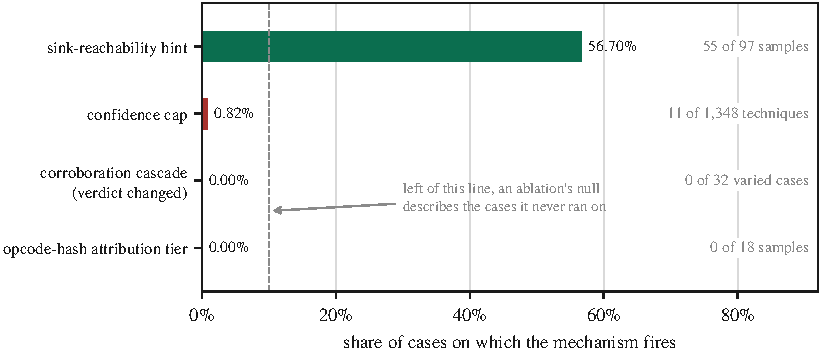
\includegraphics[keepaspectratio,alt={Figure 2: firing rate decides whether an ablation can be read at all.}]{figures/fig4-firing-rate-before-effect.pdf}}
\caption{Firing rate decides whether an ablation can be read at all.}
\end{figure}

\begin{figure}
\centering
\pandocbounded{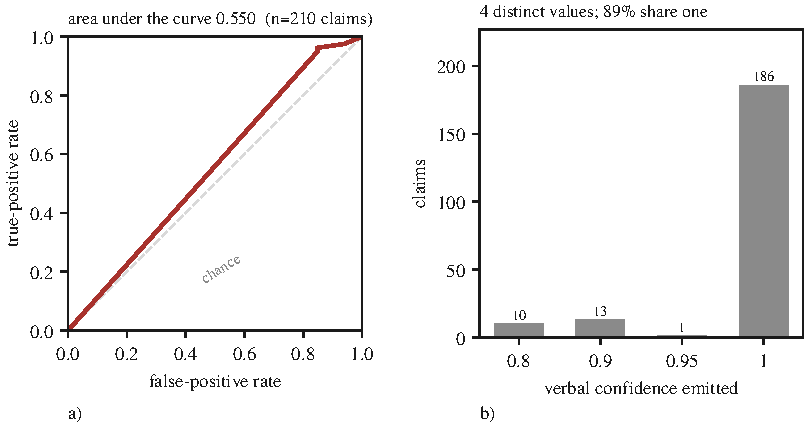
\includegraphics[keepaspectratio,alt={Figure 3: the number the gates consume barely orders anything. Panel a) is the ROC against resolved ground truth, panel b) the distribution of emitted confidence.}]{figures/fig2-confidence-discrimination.pdf}}
\caption{The number the gates consume barely orders anything. a) the ROC over \fact{confidence-n} claims against resolved ground truth, b) the confidence actually emitted.}
\end{figure}

Whether any of these mechanisms can be ablated at all depends on how often it engages, which
Table~\ref{tab:firing} and Figure~2 report. Three of the four mechanisms the architecture was built
around engage on almost nothing, so an ablation of any of them would return a null describing the
cases where the mechanism never ran. Only the sink-reachability hint clears a rate at which an
ablation carries information, which is why it is the one we ablated.

\begin{table}[!htbp]
\caption{Firing rate before effect, and the one ablation it justified. Units differ per row of the lower block and are named in the row.}\label{tab:firing}
\centering\small
\begin{tabular}{@{}
  >{\raggedright\arraybackslash}p{0.34\linewidth}
  >{\raggedright\arraybackslash}p{0.24\linewidth}
  >{\raggedright\arraybackslash}p{0.34\linewidth}@{}}
\toprule
mechanism & fires on & consequence \\
\midrule
confidence cap & \fact{cap-rate} of techniques & an ablation would measure nothing \\
sink-reachability priority hint & \fact{hint-rate} of samples (\fact{hint-fired}/\fact{hint-total}) & an ablation is interpretable and was run \\
STIX integrity pass & \fact{integrity-bundles} fresh judge bundles & reported by removal reason \\
\midrule
outcome of the hint ablation & mean $\Delta$ (on $-$ off) & 95\% CI \\
\midrule
distinct technique IDs & \fact{sink-delta-tids} & \fact{sink-ci-tids} \\
claims & \fact{sink-delta-claims} & \fact{sink-ci-claims} \\
seconds & \fact{sink-delta-seconds} & \fact{sink-ci-seconds} \\
\bottomrule
\end{tabular}
\end{table}

The hint does nothing measurable. On n=\fact{sink-pairs} pairs it is better on \fact{sink-better},
worse on \fact{sink-worse} and tied on \fact{sink-tied}, with per-pair deltas of
\fact{sink-pair-deltas}, large in both directions and cancelling. This is the fourth architectural
claim to end in a null and the last one we were in a position to test.

The result that constrains that result is that half the experiment was not scoreable. Twelve pairs
were attempted and \fact{sink-pairs} survived screening: \fact{sink-excluded-degenerate} were lost
to degenerate decode, an arm emitting \fact{degenerate-claims-min} to \fact{degenerate-claims-max}
claims across \fact{degenerate-tids-min} to \fact{degenerate-tids-max} technique IDs at ratios
\fact{degenerate-ratio-min} to \fact{degenerate-ratio-max}; \fact{sink-excluded-unattributable} were
unattributable, both arms dead with the host state needed to decide whether the pipeline or the
machine failed never recorded; and \fact{sink-excluded-incomplete} were incomplete, an arm exceeding
the \setting{630}\,s bound, which is a genuine outcome that still costs the pair. A
\fact{sink-pair-loss-rate} pair-loss rate bounds what any ablation on this pipeline can detect, and
quoting \fact{sink-delta-tids} \fact{sink-ci-tids} without it would claim a precision the instrument
does not have.

The two unattributable pairs are this paper's own retention rule recurring against it. The run
halted at \fact{halted-arms} arms and they died under host memory pressure, with
\fact{paged-out-working-set} of the model server's address space paged out, which
Section~\ref{sec:limitations} reports as a threat in its own right. We had retained per-sample
outputs, as our own rule requires; what went unrecorded was the environment the measurement ran
in. The harness now captures
\texttt{MemAvailable}, \texttt{SwapFree} and the server's resident-versus-swapped split at both ends
of every arm and the scorer screens on it, forward only, never for data already collected. Three
arms failed outright: two carried a \texttt{Connection\ error} from a restart race, meaning the
measurement never happened, and were re-run, contributing a \fact{sink-recovered-pair-delta} against
the hint; the third was the \setting{630}-second timeout, which is an outcome, and deleting an
outcome one dislikes is selection rather than repair. Running the ablation also surfaced a production
defect that \fact{test-count} passing tests did not, described as M4 in
Section~\ref{sec:failures}: on any binary rich enough to exhaust the \fact{react-step-budget}-step
ReAct budget the analyst returned zero techniques, because the salvage path received a fresh copy of
a budget it was already inside. Fixed and verified on the same sample, from
\fact{m4-fix-before-seconds}\,s to \fact{m4-fix-after-seconds}\,s and from
\fact{m4-fix-before-tids} to \fact{m4-fix-after-tids} technique IDs. The fix is partial: one sample
still exceeds the bound, and the server's own timings show generation varying from
\fact{decode-rate-fast} to \fact{decode-rate-slow} tokens/s on this hybrid recurrent architecture, so
a bounded input does not rescue a case where the tokens themselves are eight times slower than
assumed.

\subsection{The corroboration cascade does not reach the verdict}\label{sec:cascade}

The multi-layer corroboration set is the design's central claim about evidence quality. We remove
one Layer-0 source at a time and compare the bundle the analyst receives against the bundle produced
with all of them, under two conditions differing in exactly one respect: whether the removed source
was the sole owner of its techniques. Under \emph{disjoint}, where its techniques disappear because
nothing else claims them, the verdict changes in \fact{cascade-disjoint-changed} of
\fact{cascade-disjoint-arms} arms at Jaccard \fact{cascade-disjoint-jaccard}
{[}\fact{cascade-disjoint-jaccard-min}, \fact{cascade-disjoint-jaccard-max}{]} against all sources.
Under \emph{overlap}, where the techniques survive under a partner source but their corroboration
changes, it changes in \fact{cascade-overlap-changed} of \fact{cascade-overlap-arms} at Jaccard
\fact{cascade-overlap-jaccard} {[}\fact{cascade-overlap-jaccard-min},
\fact{cascade-overlap-jaccard-max}{]}. Take a technique away and the bundle loses it; leave the
technique in place and destroy the cross-domain agreement behind it, which is the thing the cascade
exists to compute, and the bundle is byte-identical.

The reason is not the one we first wrote, and the correction is M5 of Section~\ref{sec:failures}.
The judge is not what makes the bundle behave this way. The reconciliation step drops every
\texttt{attack-pattern} whose technique ID cannot be resolved and appends every cascade technique
missing from the bundle, so the cascade's set is a guaranteed subset of every bundle the system
emits whatever the judge produced. Recomputing each arm's cascade set from the same seeded fixtures
shows the bundle is exactly that set in \fact{judge-mechanism-arms} of \fact{judge-mechanism-arms}
arms, with the judge contributing zero techniques to any of them, so both conditions follow from set
arithmetic rather than from restraint. The Jaccard was the tell we missed, for the reason M5 gives.

That bound was stated rather than the stronger claim it invites, because the evidence could not
distinguish a judge whose output was unusable and wholly replaced from one that reproduced the
cascade's set exactly. The measurement has since been taken, by intercepting the reconciliation step
and recording what the model produced before the deterministic set was merged in.
Table~\ref{tab:judge} reports it on the four calls that reached that step. Three of the four
produced nothing nameable at all; the fourth named twelve techniques, every one already in the
cascade. Three quarters of the model's own attack-patterns asserted a behaviour it could not map to
a technique and were discarded. The bundle is the cascade's set wearing the judge's name.

\begin{table}[!htbp]
\caption{What the judge contributed to the artefact the analyst receives, intercepted at the reconciliation seam. Counts are techniques, over four calls.}\label{tab:judge}
\centering\small
\begin{tabular}{@{}lrr@{}}
\toprule
& total & per call \\
\midrule
attack-patterns the judge emitted & \fact{judge-capped-emitted} & \fact{judge-capped-emitted-per-call} \\
carrying a resolvable ATT\&CK ID & \fact{judge-capped-resolvable} & \fact{judge-capped-resolvable-per-call} \\
dropped, the model named no technique & \fact{judge-capped-dropped} (\fact{judge-capped-dropped-share}) & \fact{judge-capped-dropped-per-call} \\
IDs the cascade did not already hold & \fact{judge-capped-own-ids} & \fact{judge-capped-own-ids-per-call} \\
injected because the judge omitted them & \fact{judge-capped-injected} & \fact{judge-capped-injected-per-call} \\
\bottomrule
\end{tabular}
\end{table}

Half the calls never reached that step. Four of the eight timed out at the verdict ceiling, and on a
timeout the verdict tool returns a text-fallback bundle that never calls the reconciliation routine,
so the cascade is not consulted on that path at all. The timeouts are not a property of the
fixtures: the judge's \fact{judge-output-cap}-token output cap was renamed by our client library to
a parameter the local inference server does not read, so the model decoded unbounded until the caller
gave up, described as M7 in Section~\ref{sec:failures}. One such call was measured at
\fact{unbounded-decode-tokens} generated tokens and was still going.

Repeating the study with the cap fixed turns the pair into a controlled experiment, and the result
inverts this section's own conclusion. With the ceiling binding, the same four fixtures fail and the
same four succeed, the judge's share of the bundle is \fact{judge-capped-share} in both conditions,
and every number on the reconciled path is identical; what changes is only how the failure arrives,
\fact{judge-output-cap} tokens of unparseable output in three and a half minutes instead of a
ten-minute timeout. The artefact is not the same, however. The fallback builder scrapes ATT\&CK IDs
from the evidence claims and from the model's own raw response. In the uncapped condition that
response is the literal string \texttt{{[}TIMEOUT{]}} and contains no IDs, so the fallback bundle was
exactly the evidence-derived set, identical to the cascade set on all four calls. In the capped
condition it is \fact{fallback-decode-chars-min} to \fact{fallback-decode-chars-max} characters of
degenerate decode, and Table~\ref{tab:fallback} reports what then reaches the analyst.

\begin{table}[!htbp]
\caption{Techniques reaching the analyst on the text-fallback path against those the corroboration cascade held, per fixture. The last column is the set no evidence source corroborated.}\label{tab:fallback}
\centering\small
\begin{tabular}{@{}llll@{}}
\toprule
fixture & fallback & cascade & only in fallback \\
\midrule
\texttt{jhuhugit} & 32 & 20 & \textbf{12} \\
\texttt{sardonic} & 27 & 25 & \textbf{2} \\
\texttt{sliver} & 46 & 23 & \textbf{23} \\
\texttt{wannacry} & 26 & 16 & \textbf{10} \\
 \\
\bottomrule
\end{tabular}
\end{table}

\fact{fallback-only-capped} techniques reach the analyst that the corroboration cascade never held,
and none goes the other way; on one sample the bundle doubles. Because the uncapped run is a control
whose raw text provably contains no IDs, every one of them is attributable to the model's own output,
and they passed through no filter at all: not the cascade, not the reconciliation step, not the
invalid-ID filter, not the integrity pass. Checked against the \fact{attck-catalogue-size}-technique
ATT\&CK catalogue they are also real, \fact{fallback-only-capped-unique} of
\fact{fallback-only-capped-unique} unique IDs existing and none invented. That removes the easy
reading. The pipeline is not emitting hallucinated identifiers a schema check would catch; it is
emitting genuine ATT\&CK techniques that no evidence source claimed and no corroboration supports, in
the same object type and the same bundle as techniques three independent sources agreed on, with
nothing downstream to tell them apart. So the finding needs its scope stated exactly. The judge has
no influence over which techniques reach the analyst on the path where it works, and more influence
on the path where it fails than on the path where it succeeds, \fact{judge-capped-own-ids} of
\fact{judge-capped-bundle} techniques when reconciliation runs against \fact{fallback-only-capped} of
\fact{fallback-bundle-total} when it does not. The architecture suppresses the model's contribution
precisely when the model is functioning, and admits it precisely when it is not.

This replaces an earlier version of the same result, and the replacement is why we trust it. The
first pass varied three of six Layer-0 sources over fixtures carrying five techniques and reported
the verdict unchanged in \fact{weights-unchanged-superseded} of \fact{weights-arms-superseded}
cases. Two defects were found in it afterwards: the absent sources included the Sigma layer, which
fires on \fact{sigma-fires} of \fact{sigma-fires-of} samples at weight \fact{sigma-weight}, above
every static layer that study did vary; and at five techniques over six sources the round-robin
assignment left one source with nothing, so its arm matched the baseline by arithmetic rather than
by measurement. The re-run uses fixtures of \fact{weights-fixture-tids-min} to
\fact{weights-fixture-tids-max} techniques so every source carries at least three claims, includes
the Sigma layer, and adds a corroborated pair that does not involve YARA. The null survives all of
it, at \fact{cascade-overlap-arms} arms rather than \fact{weights-arms-superseded}. One
pre-registered prediction resolved in both directions: removing the tool-artifact layer should
change nothing, because it emits on YARA's cascade domain and cannot contribute corroboration, and
under overlap that is exactly right at \fact{cascade-overlap-fixtures-changed} of
\fact{cascade-overlap-fixtures} while under disjoint it is wrong at
\fact{cascade-disjoint-fixtures-changed} of \fact{cascade-disjoint-fixtures}, because there the
source solely owns its techniques. The prediction holds precisely where corroboration is the only
thing varying, which is the sharpest evidence we have that the two conditions measure what we claim.
